\documentclass[11pt,a4wide]{article}
\usepackage{verbatim}
\usepackage{listings}
\usepackage{graphicx}
\usepackage{a4wide}
\usepackage{color}
\usepackage{amsmath}
\usepackage{amssymb}
\usepackage[dvips]{epsfig}
\usepackage[T1]{fontenc}
\usepackage{cite} % [2,3,4] --> [2--4]
\usepackage{shadow}
\usepackage{hyperref}
\usepackage{graphicx}
\usepackage[english]{babel}
\usepackage{float}
\usepackage{import}
\setcounter{tocdepth}{2}
\usepackage{listings}
\usepackage{color}
\usepackage{array}


\definecolor{blue}{rgb}{0,0,0.8}
\definecolor{mygray}{rgb}{0.5,0.5,0.5}
\definecolor{mymauve}{rgb}{0.58,0,0.82}

\lstdefinestyle{mystyle}
{ 
    backgroundcolor=\color{white},   
    commentstyle=\color{blue},
    keywordstyle=\color{magenta},
    numberstyle=\tiny\color{mygray},
    stringstyle=\color{mymauve},
    basicstyle=\footnotesize,
    frame=single,
    breakatwhitespace=false,         
    breaklines=true,                 
    captionpos=b,                    
    keepspaces=true,                 
    numbers=left,                    
    numbersep=5pt,                  
    showspaces=false,                
    showstringspaces=false,
    showtabs=false,                  
    tabsize=2, 
    stepnumber=2
}

\lstset{style=mystyle}


\begin{document}

\title{Solution to Newtonian Gravity problem with many bodies \break Computational Physics-Phy905 \break Project 3}
\author{Crispin Contreras}
\date{\today}
\maketitle


\begin{abstract}
This paper discusses the numerical solution to Newtonian Gravity with different planets in our solar system. Two methods were used to solve the problem one was the Verlet method and the other one was the Runge-Kutta to the fourth order (RK4). From these two methods I found that the RK4 was more accurate and also when calculating the conservation of energy it did a better job as was expected. 
\end{abstract}



\section{Introduction}
I start by solving the the equations for Newtonian gravity. I begin with the simple Sun-Earth system and then move on to solve the Sun-Earth-Jupiter system with the Sun fixed and then the Sun-Earth-Jupiter with the Sun not fixed. Finally I model all the planets including Pluto. I used two different methods to solve this problem which are the Verlet and Runge-Kutta to the fourth order (RK4). This are just Taylor expansions and I discuss more about them in the Methods section. I test to see how stable the systems are by looking at different time steps and also increasing the time that the planets obit. Finally include my results and the conclusions that I arrived to. 

\section{Theory}
\subsection{Earth-Sun System}
I start with the Newtonian gravity which is given by $\ {\bf F} = - \frac{GM_1M_2}{r^2} {\bf \hat{r}}$. Here G is the gravitational constant, r is the distance between the bodies, and M represents the mass. I decided to work in Cartesian coordinates so I use 
\begin{equation}
\begin{split}
    {\bf \hat{r}} = cos(\theta){\bf \hat{x}} + sin(\theta){\bf \hat{y}}\\
    x=rcos(\theta), \hspace{0.3cm} y=rsin(\theta) \hspace{0.3cm} r = \sqrt{x^2 + y^2}
\end{split} 
\end{equation}
Where $\ \theta$ is just the polar angle. Now using equation (1) I break the equation for gravitation into Cartesian coordinates 
\begin{equation}
\begin{split}
	F_x = -\frac{GM_1M_2}{r^3}x \\
	F_y = -\frac{GM_1M_2}{r^3}y 
\end{split}
\end{equation}
With equation (2) now I can start setting up the equations of motions for the planets. I start with the Earth-Sun system where I treat the Sun as stationary so I use it as the origin. I start with the equations of motion, for simplicity I will only do the x coordinate since the only thing that changes in the others is the coordinate itself.  
\[
	M_{Earth}\frac{d^2x}{dt^2} = -\frac{GM_{Earth}M_{Sun}}{r^3}x
\]
I will simplify this equation further by introducing a new set of units for the G and mass. The Earth's orbit around the sun is almost circular around the Sun so for this type of motion the force is given by 
\[
	F =\frac{M_{Earth}v^2}{r}=\frac{GM_{Sun}M_{Earth}}{r^2}
\]
from this equation we can get rid of the gravitational constant G and mass of the sun to replace it by 
\begin{equation}
	v^2r=GM_{Sun}=4\pi^2 (\frac{AU^3}{yr^2})
\end{equation}
with this transformation now we can use the astronomical units (AU) for length and year (yr) for time. The mass of the Sun is then one. Now the equation of motion for the earth reads 
\begin{equation}
\begin{split}
	F_x = \frac{d^2v_x}{dt^2} = -\frac{4\pi^2}{r^3}x \\
	\frac{dx}{dt}=v_x
\end{split}
\end{equation}
The equation for the y coordinate is the same except the x is replace by y. 
\subsection{Three Body Problem}
I start with a simplified version of the three body problem. In this case I model the Sun, Earth, and Jupiter but I will keep the Sun fixed. For the Earth the only thing that changes now is that it feel the force from Jupiter. The force now reads
\begin{equation}
	F_x^{Earth}= \frac{dv_{x_E}}{dt} =-\frac{4\pi^2}{r_{ES}^3}x_E - \frac{4\pi^2(M_{Jupiter}/M_{Sun})}{r_{EJ}^3}(x_E -x_J)
\end{equation}
where now include the coordinates for Jupiter, $\ r_{EJ}$ is the distance between the Earth and Jupiter, and $\ r_{ES}$ is the distance between the Earth and the Sun. Here $\ x_J$ is the position of Jupiter and $\ x_E$ is the position of the Earth and M represents the mass of the bodies. The same equation for (5) is obtained for y  except the x is replace by either y. $\ r_{EJ}$ is given by 
\[
	r_{EJ}=\sqrt{(x_E -x_J)^2+(y_E -y_J)^2+}
\]
For Jupiter I obtain the equation 
\begin{equation}
	F_x^{Jupiter}= \frac{dv_{x_J}}{dt} =-\frac{4\pi^2}{r_{JS}^3}x_J - \frac{4\pi^2(M_{Earth}/M_{Sun})}{r_{EJ}^3}(x_J -x_E)
\end{equation}
here $\ r_{JS}$ is the distance between Jupiter and the Sun, in order to get the y coordinate I just replace x by y.  

Now to do the full three body problem I will allow the Sun to move instead of being fixed. This means that the origin of the system is now the center of mass of the three bodies. I give the equation for the Sun 
\begin{equation}
	F_x^{Sun}= \frac{dv_{x_S}}{dt} =-\frac{4\pi^2(M_{Jupiter}/M_{Sun})}{r_{JS}^3}(x_S- x_J) - \frac{4\pi^2(M_{Earth}/M_{Sun})}{r_{SE}^3}(x_S -x_E)
\end{equation}
for equations (5) and (6) the only thing that gets modified is the term $\ x_J$ which goes to $\ (x_J -x_S)$ and $\ x_E$ which goes to $\ (x_E -x_S)$, the same thing occurs for the y variable. With equations (5),(6),and (7) now I can solve the three body problem in two dimensions. 
	
Finally to model the all the planets of the solar system and Pluto, I keep the sun fixed for simplicity. In general the equation is given by 
\begin{equation}
	F_x^j = -\frac{4\pi^2}{r_{jS}^3}(x_j-x_S) -4\pi^2\sum_{ i=1,j\neq i}^9{\frac{M_i/M_{Sun}}{r_{ji}^3}(x_j-x_i)}
\end{equation} 
here j and i can take on the values $\ j,i =1,2,3...9$ and they represent how far the planet is from the Sun. For example Mercury will be 1, Venus 2, and so on. Now that I have all the equations setup I can move on to describe the methods. 

\begin{equation}
\left(\begin{array}{ccccccc}
 	d_1& e_1& 0& \dots& \dots&  \dots &0\\
    e_1& d_2& e_1& 0& \dots& \dots &0 \\
    0& e_1 &d_3 & e_1 & 0 & \dots &0\\
    \dots& \dots   & \dots &\dots   &\dots & \dots &\dots\\
    \dots &\dots &\dots &\dots &\dots &\dots &\dots \\
    0 &\dots   &\dots  &\dots &e_1 &d_{n -1}& e_1 \\
    0 &\dots    &\dots  &\dots & 0  & e_1 & d_n \\
    \end{array} \right)   \left(\begin{array}{c}
    											u_1 \\
    											u_2 \\
    											\vdots \\ \vdots \\ \vdots \\ 
    											u_n
    			                \end{array}\right) = \lambda \left(\begin{array}{c}
    											u_1 \\
    											u_2 \\
    											\vdots \\ \vdots \\ \vdots \\ 
    											u_n
    			                \end{array}\right)        
\end{equation}

\section{Methods}
Two methods were implemented two solve the equations above. I used the Verlet method which has an accuracy of . I also used the Runge-Kutta 4 which is more precise than the Verlet but has more floating point operations. The basic idea behind these two methods is to use a Taylor expansion and for each one have a different truncation. I take much of the derivations from [1]. 
\subsection{Verlet Method}
In order to derive the algorith for the verlet I will start by using Newton's second law  in one dimension which reads
\[
	m\frac{d^2x}{dt^2} = F(x,t) 
\]
this can be rewritten in terms of couple equation such that 
\[
	
\]
The Jacobi method consists of using many similarity transformation to reduce a matrix into diagonal form. In this case the matrix is $\ {\bf A}$. This method is chosen since doing a determinant for large matrices is impractical. The similarity transformation is defined by 
\[
	{\bf B} ={\bf S^{T}AS}
\]
The $\ {\bf S}$ has the following property $\ {\bf S^T}={\bf S^{-1}}$. In our case the similarity transformation is defined by 
\[
	s_{kk} =s_{ll}=cos(\theta), \hspace{0.3cm} s_{kl}=-s_{lk}=-sin(\theta), \hspace{0.3cm} s_{ii} =1 , \hspace{0.3cm} 
	 i \neq l \hspace{0.3cm} i \neq k
\]
the other terms are zero. The results for the $\ {\bf B}$ matrix are 
\begin{equation}
\begin{split}
 	b_{ik}=a_{ik}cos(\theta) -a_{il}sin(\theta), \hspace{0.3cm} i \neq k, \hspace{0.3cm} i \neq l \\
 	b_{il}=a_{il}cos(\theta)+a_{ik}sin(\theta), \hspace{0.3cm} i \neq k, \hspace{0.3cm} i \neq l \\
 	b_{kk}=a_{kk}cos^2(\theta) -2a_{kl}cos(\theta)sin(\theta) +a_{ll}sin^2(\theta), \hspace{0.3cm} \\
 	b_{ll}=a_{ll}cos^2(\theta)+2a_{kl}cos(\theta)sin(\theta) +a_{kk}sin^2(\theta), \hspace{0.3cm} \\
 	b_{kl}=(a_{kk} - a_{ll})cos(\theta)sin(\theta) +a_{kl}(cos^2(\theta) -sin^2(\theta))   \\
\end{split}
\end{equation}
The recipe is the to chose $\ \theta$ so that all non-diagonal elements $\ b_{kl}$ become zero. We require that $\ b_{kl}$ =$\ b_{lk}$ = 0 which then leads to 
\[
	b_{kl}=(a_{kk} - a_{ll})cos(\theta)sin(\theta) +a_{kl}(cos^2(\theta) -sin^2(\theta))=0	
\]
if $\ a_{kl}=0$ then this leads to $\ cos(\theta)$ = 1 and $\ sin(\theta)$ =0. To solve the equation above we define $\ tan(\theta)=t =\frac{s}{c}$ , $\ sin(\theta) =s$, $\ cos(\theta) = c$, and use the trigonometric identity $\ cos(2\theta)=\frac{1}{2(cot(\theta)-tan(\theta))}$ to obtain
\[
	cos(2\theta)=\tau= \frac{a_{ll} -a_{kk}}{2a_{kl}}
\]
using the trigonometric identity we obtain 
\[
	t^2 +2\tau t- 1=0
\]
resulting in 
\[
	t = -\tau \pm \sqrt{1+\tau^2}
\]
and we can obtain c and s by using trigonometric tricks 
\[
	c = \frac{1}{\sqrt{1+t^2}}
\]
and $\ s=tc $. In order to get the off-diagonal terms to be equal to zero or in our case  $\ \geq $ $\ 10^{-8}$ we have to complete many similarity transformations until this occurs. In order to figure this out we look at the Frobenius norm which is defined as 
\[
	||{\bf A}||_F = \sqrt{\sum_{i=1}^n \sum_{j=1}^n |a_{ij}|^2}
\]
One of the important properties of the Frobenius norm is that it's the same after similarity transformations. This property will be  used in the Jacobi algorithm. Solving the quadratic equation we find that $\ |\theta| \leq \frac{\pi}{4}$ having this property then leads to a minimization of the difference between $\ {\bf A}$ and $\ {\bf B}$ since 
\[
||{\bf B}-{\bf A}||_F^2=4(1-c)\sum_{i=1,i\ne k,l}^n(a_{ik}^2+a_{il}^2) +\frac{2a_{kl}^2}{c^2}.
\]
To summarize, the Jacobi methods consists of many similarity transformations in order to decrease the value of the off diagonal elements. This can be done by looking at the  norm. This algorithm was implemented in C++ and it's show below in listing 1. 

\lstinputlisting[language =C++,firstline=113, lastline=143, caption = This shows how the Jacobi method was implemented. The rotate function is called here and it's responsible for carrying out the operation in (6).]{"/home/quetzalcoatl/Computational_Physics_work/Project2/Code/Project2.cpp"}
\subsection{Runge-Kutta 4 method}


\section{Results}
\subsection{Single Electron} 

The Jacobi algorithm was implemented in C++ according to section 3. This was then compared to the Armadillo's eigenvalue solver $\ eig-sys()$ to make sure it was working properly. The energy eigenvalues are know and were discussed in the theory sections. Their values 3,7,and 11 were used for calibration for getting the $\ \rho_{max}$. By trial and error we found that the best value for the three lowest states was $\ \rho_{max} = 5$. The results for the eigenvalues and computational times are shown in table 1 below. From table 1 we can see that as the value of n increases the eigenvalues get closer to the correct values. Table 1 also shows the number of iterations that the Jacobi method must make in order for the off-diagonal terms to be$\ \leq 10^{-8}$. From table 1 we can also estimate the number of similarity transformations in order to get the off-diagonal terms to $\ 10^{-8}$ which is roughly $\ 1.7n^2$. Finally we made a plot using matplolib for the corresponding three lowest state which is shown in figure 1. In this case we made sure the wavefunctions were normalized as $\ \int_0^\infty |u(\rho)|^2d\rho$. This was done by approximating the integral as a set of rectangles (like a histogram) and using the values of the normalized eigenfunctions as the height and the width from h we can calculate the area.The the integral is just 
\[
	\ \int_0^\infty |u(\rho)|^2d\rho \approx h\left(\sum_{j=1}^n |u_{j}|^2 \right)
\]
From this then we can get the normalized eigenfunctions by multiplying by $\ \frac{1}{h}$. This same procedure is done for the two electron case. 

\begin{figure}[H] 
\centering
%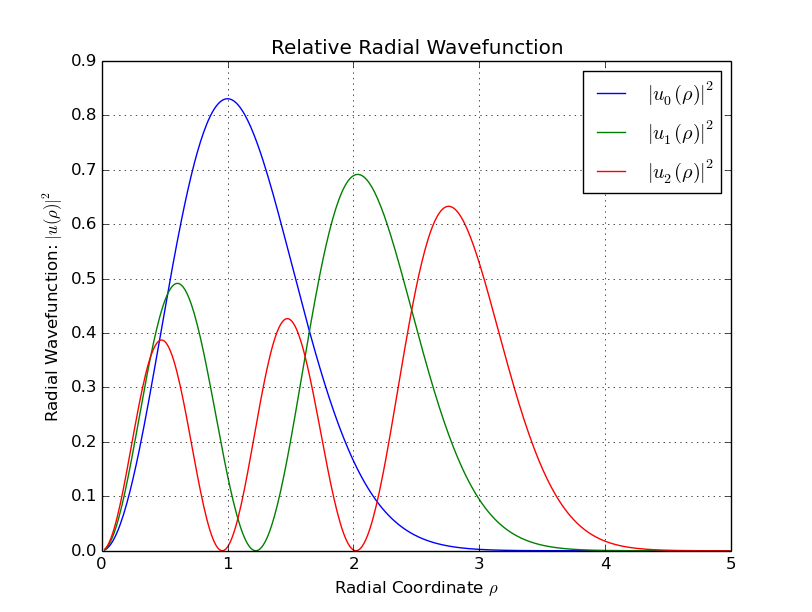
\includegraphics[width=100mm]{NI.png}
\caption{ Plot of the radial wavefunctions for the three lowest energies. The eigefunctions were normalized and we used $\ \rho_{max}$ = 5 and n=400.\label{overflow}}
\end{figure}
\begin{table}[H]
\centering
\label{my-label}
\begin{tabular}{| m{2cm} | m{3cm} | m{3cm} | m{3cm} | m{3cm} |}
 \cline{1-5}
  Grid Points, n&  3 Lowest Energy Eigenvalues For Jacobi, $\ \lambda$&  Calculation Time, $\ T_{Ja}$ [s]&   Calculation Time, $\ T_{arma}$ [s]& Number of iterations \\ \cline{1-5}
 50&  2.9969, 6.9850, 10.9634&  0.01653& 0.001274& 4040\\ \cline{1-5}
 100& 2.9992, 6.9962, 10.9908&  0.22181& 0.003996& 16475\\ \cline{1-5}
 200& 2.9998, 6.9990, 10,9978&  3.67701& 0.021410& 66828\\ \cline{1-5}
 300& 2.9999, 6.9996, 10.9991&  17.7895& 0.069452& 150798\\ \cline{1-5}
 350& 2.9999, 6.9997, 10.9994&  34.5932& 0.083118& 205757\\ \cline{1-5}
 400& 3.0000, 6.9998, 10.9996&  57.7010& 0.122340& 269021\\ \cline{1-5}
\end{tabular}
\caption{This table shows the number of grid points, the eigenvalues, Computational time, and the number of iterations. From here we can interpolate the number of similarity transformations needed to reach $\ 10^{-8}$.  }
\end{table}

\subsection{Two Interacting Electrons}
We use the same code for the single electron and modify it to include the Coulomb interaction. To see if the values are correct we use [2] and the values given by this source. This is shown in table 2.
\begin{figure}[H]
\centering
%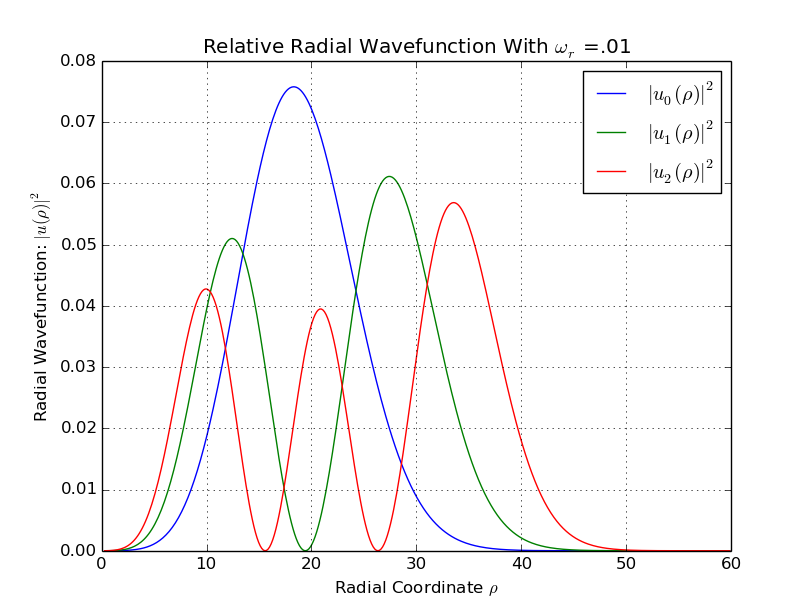
\includegraphics[width=100mm]{I_01.png}
%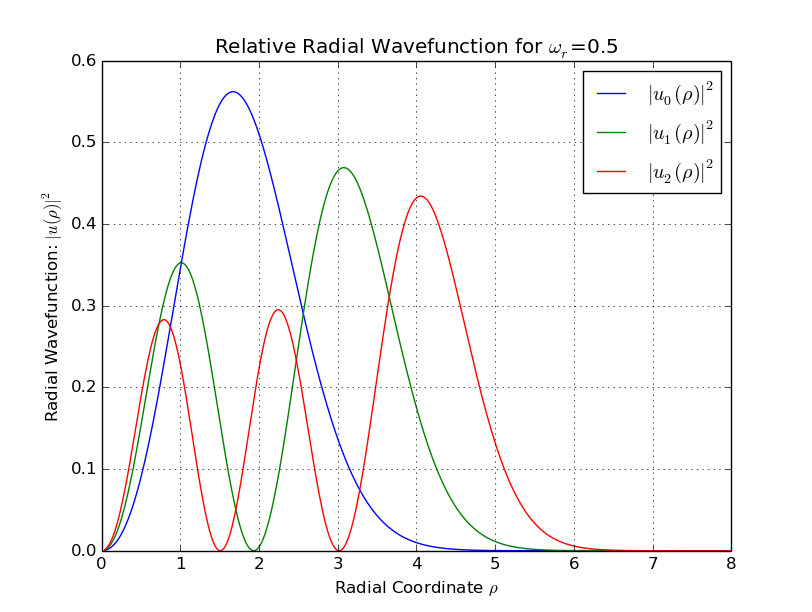
\includegraphics[width=100mm]{I_5.png}
\caption{This figure show the normalized eigenfunction for $\ \omega_r$ =0.01 and $\ \omega_r$=0.5. The values for $\ \rho_{max}$ are 60 and 8 repectively witn $\ n=400$. \label{overflow}}
\end{figure}
\begin{figure}[H]
\centering
%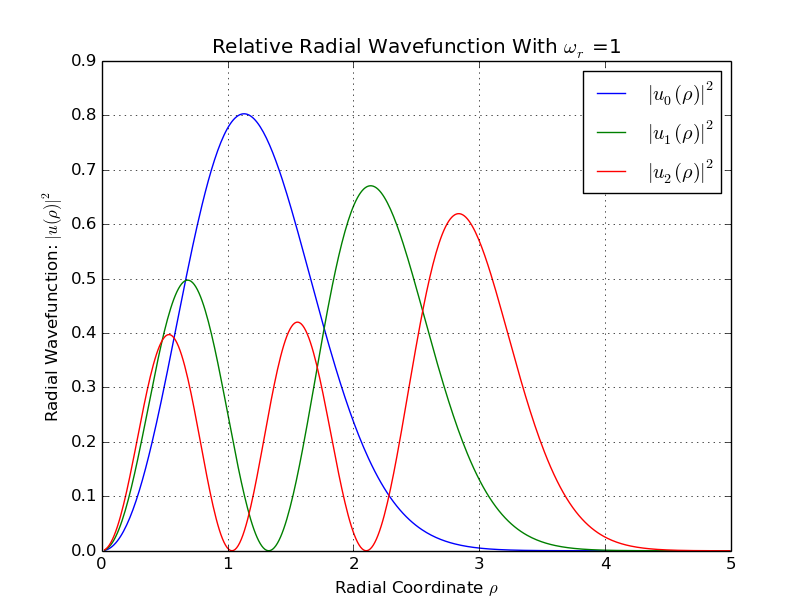
\includegraphics[width=100mm]{I_1.png}
%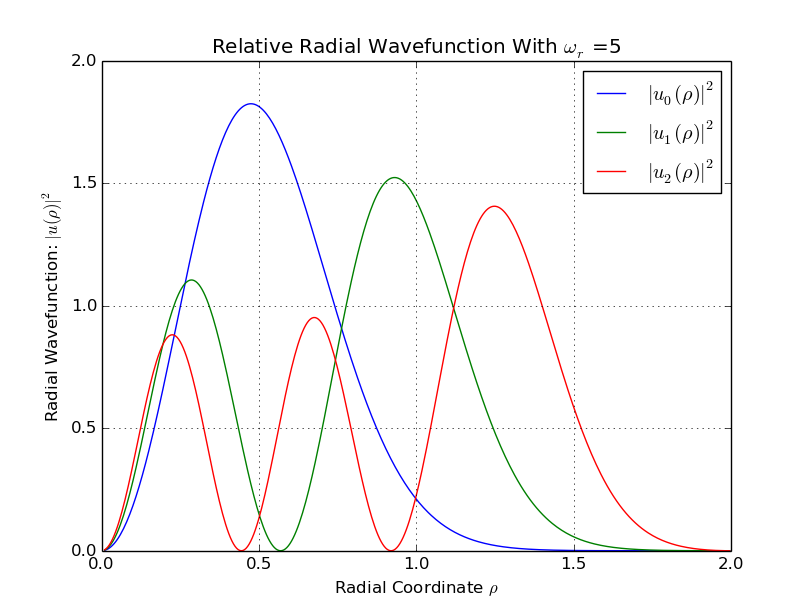
\includegraphics[width=100mm]{I_50.png}
\caption{This figure show the normalized eigenfunction for $\ \omega_r$ =1 and $\ \omega_r$=5. The values for $\ \rho_{max}$ are 8 and 2 repectively witn $\ n=400$. \label{overflow}}
\end{figure}

\begin{table}[H]
\centering
\label{my-label}
\begin{tabular}{| m{3cm} | m{3cm} | m{3cm} | m{3cm} |}
 \cline{1-4}
 Oscillator Frequency $\ \omega_r$&  Ground State Energy Eigenvalues, $\ \lambda$&  [2] Approximate Formula, 2$\ \epsilon'$&  [2]improved formula, 2$\ \epsilon'_int$ \\ \cline{1-4}
 0.01&  0.1058& 0.1050& --\\ \cline{1-4}
 0.05&  0.3500& 0.3431& 0.3500\\ \cline{1-4}
 0.25&  1.2500& 1.1830& 1.2500\\ \cline{1-4}
 0.5&  2.2300&  2.0566& --\\ \cline{1-4}
 1&  4.0578&    3.6219& --\\ \cline{1-4}
 5&  17.4485&   14.1863& --\\ \cline{1-4}
\end{tabular}
\caption{Values for the frequency $\ \omega_r$ and the energy eigenvalues. Also shown are the results from [2] which are the accepted values for the energies. We used these to make sure the algorithm was working correctly.}
\end{table}

\section{Discussion}
The implementation of the Jacobi algorithm produced good results as shown in table 1 since they have good agreement with the know energy values. From table 1 we obtain that approximately $\ 1.7n^2$ similarity transformations are needed to get the off-diagonal terms close to zero. This is less since our matrix is tridiagonal, for a full matrix a total of $\ 3n^2$ to $\ 5n^2$ transformations are needed[1]. We also saw that the Jacobi method has a very large computational time as opposed to the Armadillo's eigenvalue solver. 

In trying to get reasonable results the biggest problem with this algorithm was determining the value of n and $\ \rho_{max}$. This took some time since it was done by trial and error. Although when I figured out one of the values it was easier to determine the others by changing $\ \rho_{max}$ a bit. In order to start analyzing the interacting case we needed to use [2] to make sure the code was working correctly. For this I used the values for $\ \omega_r $=0.25 and 0.05 and compared to [2]. As shown in table 2 our results show that our program was working correctly. In addition to this I also checked that the norm of the lowest eigenvectors were equal to 1. This is because the Frobenius norm is no affected by transformations. Again my results shows that this was true. These were the "unit test" that I implemented to make sure my code was working correctly.

Finally I discuss the physics of plots. I use figure 1 as basis and compared to the other plots. The main result is that the eigenfunctions were stretch or squeezed depending on the size of $\ \omega_r$. For small values of $\ \omega_r$ we can see that eigenfunctions get stretched in the horizontal direction while for large values they get squeezed. We see that the electrons are further apart from each other when we include the interaction which is what is expected. 

\section{Conclusion}
The Jacobi algorithm was implemented and we found that it had a very large computational time compared to Armadillo's eigenvalue solver. Additionally it was a bit time consuming figuring out what the best value for $\ \rho_{max}$ was and similarly for n. The only way to do this was by trial and error. For the interacting case we found that the electrons get more spread out and this is what is expected since they have the same charges. The results for the interacting case were in agreement with [2] since the eigenvalues agreed. 

\section{References}
[1] M. Hjorth-Jensen.~Computational Physics, Lecture Notes Spring 2016.\break
[2] M.~Taut.Two electrons in an external oscillator potential: Particular analytical solutions of a coulomb correlation problem. Phys. Rev. A. 48, 3561-3566 (1993)

\section{Code Attachment}
\lstinputlisting[language =C++]{"/home/quetzalcoatl/Computational_Physics_work/Project2/Code/Project2.cpp"}

\end{document}

